\documentclass[%
 %reprint,
 %twocolumn,
 %superscriptaddress,
 %groupedaddress,
 %unsortedaddress,
 %runinaddress,
 %frontmatterverbose,
  preprint,
 showpacs,
 showkeys,
 preprintnumbers,
 %nofootinbib,
 %nobibnotes,
 %bibnotes,
 amsmath,amssymb,
 aps,
 prl,
 %  pra,
 % prb,
 % rmp,
 %prstab,
 %prstper,
  longbibliography,
 %floatfix,
 %lengthcheck,%
 ]{revtex4-1}

%\usepackage{cdmtcs-pdf}

\usepackage{amssymb,amsthm,amsmath}


\theoremstyle{definition}
\newtheorem{definition}{Definition}
\newtheorem{theorem}{Theorem}
\newtheorem{conjecture}{Conjecture}

\theoremstyle{remark}
\newtheorem*{motivation}{Motivation}
\newtheorem*{note}{Note}

\usepackage{tikz}
\usepackage[breaklinks=true,colorlinks=true,anchorcolor=blue,citecolor=blue,filecolor=blue,menucolor=blue,pagecolor=blue,urlcolor=blue,linkcolor=blue]{hyperref}
\usepackage{graphicx}% Include figure files
\usepackage{url}

\usepackage{xcolor}

\begin{document}


\title{Unscrambling the Quantum Omelette}

%\cdmtcsauthor{Karl Svozil}
%\cdmtcsaffiliation{Vienna University of Technology}
%\cdmtcstrnumber{407}
%\cdmtcsdate{September 2011}
%\coverpage

\author{Karl Svozil}
\affiliation{Institute for Theoretical Physics, Vienna
    University of Technology, Wiedner Hauptstra\ss e 8-10/136, A-1040
    Vienna, Austria}
\affiliation{Dipartimento di Scienze Pedagogiche e Filosofiche, Universit\'a  di Cagliari,\\
 Via Is Mirrionis, 1, I-09123, Cagliari, Sardinia, Italy}
\email{svozil@tuwien.ac.at} \homepage[]{http://tph.tuwien.ac.at/~svozil}
\thanks{Contribution to the 11th Biennial  International Quantum Structure Association  (IQSA) Meeting
"Quantum Structures Cagliari 2012," 23 - 27 July - Cagliari (Italy)}

\pacs{03.65.Ta, 03.65.Ud}
\keywords{quantum  measurement theory, mixed state, quantum probability}
%\preprint{CDMTCS preprint nr. 407/2011}

\begin{abstract}
Despite its excessive success in predicting experimental frequencies and certain single outcomes,
``Born's quantum mechanics'' is haunted by several conceptual and technical issues; among them
(i) the (non-)existence of measurement in an environment globally determined by a unitary evolution;
(ii) what constitutes a pure quantum state;
(iii) the (non-)existence of mixed states;  as well as
(iv) the assumption that all counterfactual observables exist.
Many of these conceptual difficulties can be overcome by assuming that only a single pure state (context) exists;
and that the quantum evolution ``permutes'' this state.
\end{abstract}

\maketitle

The following rather ``iconoclastic'' reconstruction of quantum mechanics applies to the quantum formalism
as outlined by von Neumann \cite{v-neumann-49}.
It will most likely survive this theory
because the definitions, conventions and results presented apply to a reversible (indeed, bijective)
state evolution,
which amounts to permutations of elements in some state space.

Epistemologically, in particular from a system science perspective,
physical perception is necessarily self-referential,
and there is no feasible ``point outside'' from which we might be capable of
obtaining an ``objective'' ontology:
all physical observations are inevitable intrinsic,
recorded by ``embedded observers.''
Intrinsic epistemology has a long tradition \cite{bos1,toffoli:79,svozil-94}.
For instance, Poincar\'e and Einstein considered
procedures for establishing temporal simultaneity,
and space-time frames in general, which amounted to conventions utilizing
strictly operational means -- utilities that are accessible
from within the system alone, without any reference to
extrinsic knowledge \cite{Galison-2003,casar-poincare-convention}.


At the most fundamental level (of resolution),
the quantum phenomena (as everything empirical), need to be (re-)constructed
from mere {\em detector clicks} alone -- that is, from discrete, dichotomic ``bit-like'' events.
(Continuity is an idealistic concept which is not operational.)
Any inductive construction of a representation of a universe entirely from ``physical signals''
and, in particular, from detector clicks, is a subtle epistemic and physical task \cite{sum-3,wheeler-89}
involving explicit and implicit conventions and assumptions.
As we do not possess any direct access to the
system other than these clicks  we have to be careful in ascribing physical properties and existence
of anything \cite{stace1}.
Indeed, it must be expected that we are deceived
by our own preconceptions, implicit conventions, and subjective expectations and projections.
Jaynes called this
the ``Mind Projection Fallacy'' \cite{jaynes-89,jaynes-90}, pointing out that
{\em ``we are all under an ego-driven temptation to project our private
thoughts out onto the real world, by supposing that the creations of one's own imagination are real
properties of Nature, or that one's own ignorance signifies some kind of indecision on the part of
Nature.''}
I believe that this ``over-interpretation of empirical data''
is at the heart of many misconceptions
about quantized systems.

Thereby metaphysical ``guiding principles''
such as personal, subjective preferences [eg., towards (in)determinism],
compactness of representation (Occam's razor),
symmetry or beauty must be applied with greatest caution.
They might even become deceptive,
blocking our comprehension of the bigger picture.
We have to be constantly aware that the contemporary peers have no certainty
about which research program will eventually turn out to be progressive
\cite{lakatosch}.

A typical preconception is a ``space-time theater'' in which detector clicks occur.
Alas, it might not be unreasonable to obtain space-times the ``other way round''
-- the events and observations
should facilitate the construction of space-time frames
through fully disclosed conventions \cite{Knuth-Bahreyni}.
In such a scheme, ``quantum nonlocality'' might just turn out to be an artifact of an
outdated ``classical'' preconception of space-time.
The price for this total operationalization of space-time would be a very delicate
fabric of space-time in which not even the dimension can be expected to be constant \cite{sv1}, and
distinctiveness and connectedness might be very different from classical relativity.

Another such preconceived preference appears to be ``quantum contextuality,''
for the obvious reason that this concept has neither any direct empirical test
(all published experiments use indirect methods; mostly they just record violations of Bell-type inequalities \cite{svozil:040102}),
nor is quantum contextuality a necessary consequence of any theorem based on quantum theory.
Still another mind projection fallacy maybe the claim of indeterminism in Nature \cite{born-26-1,born-26-2},
which is provably unprovable.

In what follows a critical re-evaluation of quantum theory
is attempted.

\begin{definition}[State, observable]
A (pure) physical {\em state} is characterized by the maximal information encodable into a physical system.

More specifically, a state is a maximal set of mutually exclusive
(if one fires all the others do not fire), dichotomic (``click--no click''),
co-measurable detector {\em observables}
${\frak A} =\{\textsf{\textbf{A}}_1,\textsf{\textbf{A}}_2,\ldots , \textsf{\textbf{A}}_n\}$;
together with a two-valued probability measure (truth-value) $P_i$, $1 \le i \le n$, thereon.
$P_i$ assigns
strictly one of these observables $\textsf{\textbf{A}}_i$,
associated with the detector
that ``fires,'' the value $P_i(\textsf{\textbf{A}}_i)=1$;
and all the other $n-1$ observables $\textsf{\textbf{A}}_{j\neq i}$, $1 \le j \neq i \le n$,
whose associated $n-1$ detectors ``do not fire,''  the value $P_i(\textsf{\textbf{A}}_{j\neq i})=0$.
\end{definition}

\begin{definition}[Quantum state representation]
A quantum state can be represented by an orthonormal basis of a Hilbert space.
Equivalently, a state can be identified with the associated unitary operator,
block, subalgebra, or maximal operator.
\end{definition}


\begin{motivation}
The $i$th observable $\textsf{\textbf{A}}_i$
can represented by a vector $\vert i \rangle$ \cite{mermin-07}
encoded by the tuple
$\left(\delta_{1i},  \ldots , \delta_{ni} \right)$
of coordinates with respect to the Cartesian standard basis
${\frak B} = \left\{(1,0,\ldots ,0),\ldots , (0,\ldots 0,1)\right\}$
of an $n$-dimensional vector space.
Thus, the $i$th observable $\textsf{\textbf{A}}_i$ of ${\frak A}$
can be identified with the $i$th element
(called ``primitive basis element'' by t'Hooft \cite{tHooft1990471})
of ${\frak B}$.


Thereby, the set of co-measurable, dichotomic detector observables
${\frak A}$
can be identified with the orthonormal basis
${\frak B}$.
Equivalently,
${\frak A}$ can be identified with
\begin{itemize}
\item[(i)]
the {\em set of orthogonal projectors} ${\frak E}
=\left\{ \textsf{\textbf{E}}_i \mid \textsf{\textbf{E}}_i   =\vert i \rangle \langle i \vert ,
1\le i \le n
\right\}$,
where $\langle i \vert$ is the vector in the dual base obtained by transposing  $\vert i \rangle$;
and $\vert i \rangle \langle i \vert$ is obtained by the dyadic product, representable as
diagonal matrix $\textrm{diag} \left(\delta_{1i},  \ldots , \delta_{ni} \right)$;
\item[(ii)]
the {\em maximal operator} composed by the spectral sum
$\textsf{\textbf{M}}=\sum_{i=1}^n \lambda_i \textsf{\textbf{E}}_i$,
with mutually distinct eigenvalues $\lambda_i \neq \lambda_j$ for all $1\le i\neq j \le n$;
\item[(iii)]
the {\em unitary operator} composed by the spectral sum \cite{Schwinger.60}
$\textsf{\textbf{U}}=\sum_{i=1}^n \textsf{\textbf{E}}_i$;
\item[(iv)]
some block and subalgebra in the usual quantum logical meaning
as constituents of quantum logic \cite{harding-navara-subalgebras}.
\end{itemize}

Note that no distinction is being made between observables and states.
\end{motivation}

\begin{definition}[Quantum probabilities]
The convex hull \cite{Henk-Ziegler-polytopes} of ${\frak B}$
%  $$P = \textrm{conv}({\frak B})
%  \stackrel{{\tiny \textrm{ def }}}{=}
%  \left\{ \left.
%  \sum_{i=1}^n   p_i(\textsf{\textbf{A}}_i) \textsf{\textbf{A}}_i
%  \right|
%  \left( p_i \in [0,1] \right)
%  \wedge
%  \left(
%  \sum_{i=1}^n   p_i(\textsf{\textbf{A}}_i) =1
%  \right)
%  \right\}$$
yields a convex polytope
representing all (quasi-classical) probability measures $P$ on
${\frak A}$
\cite{Boole-62,pitowsky}.

In Hilbert space quantum mechanics,
for larger than two dimensions,
the hypothetical assumption of the co-existence
of (the continuity of) all collections of systems of detector observables (such as ${\frak A}$ discussed earlier)
the quasi-classic probability measures on single states can be extended to
non-co-measurable observables by Gleason's theorem \cite{r:dvur-93},
thereby yielding's the Born rule for quantum probabilities.
\end{definition}


\begin{note}
We take the co-existence of states which are not co-measurable as a physically unjustified {\it artifact} of Hilbert space quantum mechanics;
because operationally only a single basis (context, subalgebra, block, maximal operator, unitary operator)
can be fixed.

Already Kochen and Specker realized this issue which they circumvented by allowing -- in distinction to the Birkhoff-von Neumann approach to quantum logic
\cite{birkhoff-36,bell-cas,pulmannova-91} --
 only operations among co-measurable observables,
resulting in ``partial algebras'' \cite{kochen3}.
However, in order to derive nontrivial results, they allowed the ``pasting'' of subalgebras across link observables,
thereby involving observables which are not co-measurable.

The co-existence of not co-measurable, that is, not simultaneously operational quantities, somehow reflects the ``experimental experience'' of
{\em omni-measurability} and {\em omniscience}:
``measurements'' of (a potential, counterfactual continuity of) observables (states) yield ``outcomes'' or ``results;'' even when the system has been prepared in a single (different) state.
Note that in no way is there a guarantee that these measurement outcomes solely reflect genuine properties of the measured object.

Diagrammatically, Fig.~\ref{2012-psiqm-v2} depicts the continuity of such non-existing ``phantom observables'' forming  ``phantom contexts'' (or ``phantom states'') can be illustrated by a
``star shaped'' Greechie diagram representation of a configuration of blocks in three dimensional Hilbert space
with overlaid two-valued measure. (For other reasons, this star-shaped configuration has also been
discussed in a recent publication of
Abbott, Calude, Conder and the author \cite[Fig.~2]{2012-incomput-proofsCJ}.)
\end{note}

\begin{figure}[h]
\begin{center}
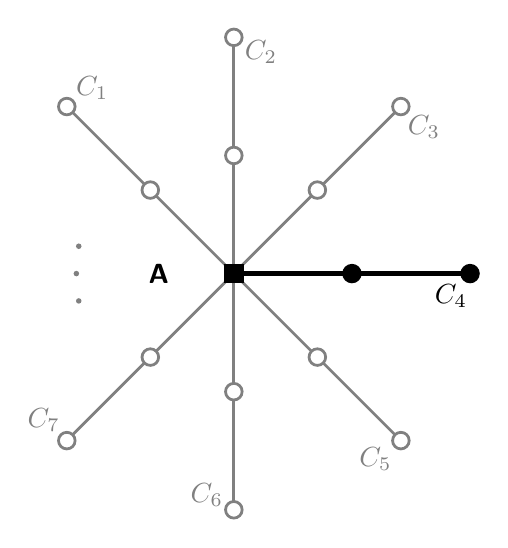
\begin{tikzpicture}
\tikzstyle{every path}=[line width=1pt]
\tikzstyle{every node}=[draw,line width=1pt,inner sep=0]

\tikzstyle{c1}=[rectangle,minimum size=6]

\tikzstyle{d1}=[circle,draw=none,fill,minimum size=2]

\tikzstyle{l7}=[draw=none,circle,minimum size=45]

\draw[gray] (0:0) -- (135:3)
	coordinate[c1,at start] (0)
	coordinate[c1,circle,midway,fill=white] (1)
	coordinate[c1,circle,at end,fill=white,label=35:$C_1$] (2);

\draw[gray] (0.center) -- (90:3)
	coordinate[c1,at start] (0)
	coordinate[c1,circle,midway,fill=white] (3)
	coordinate[c1,circle,at end,fill=white,label=350:$C_2$] (4);

\draw[gray] (0.center) -- (45:3)
	coordinate[c1,at start] (0)
	coordinate[c1,circle,midway,fill=white] (5)
	coordinate[c1,circle,at end,fill=white,label=305:$C_3$] (6);

\draw[gray] (0.center) -- (315:3)
	coordinate[c1,at start] (0)
	coordinate[c1,circle,midway,fill=white] (9)
	coordinate[c1,circle,at end,fill=white,label=215:$C_5$] (10);

\draw[gray] (0.center) -- (270:3)
	coordinate[c1,at start] (0)
	coordinate[c1,circle,midway,fill=white] (11)
	coordinate[c1,circle,at end,fill=white,label=170:$C_6$] (12);

\draw[gray] (0.center) -- (225:3)
	coordinate[c1,at start] (0)
	coordinate[c1,circle,midway,fill=white] (13)
	coordinate[c1,circle,at end,fill=white,label=125:$C_7$] (14);

\draw[black,line width=2pt] (0.center) -- (0:3)
	coordinate[c1,fill,at start] (0)
	coordinate[c1,circle,fill,midway] (7)
	coordinate[c1,circle,fill,at end,label=260:$C_4$] (8);

\coordinate[l7,label=180:$\textsf{\textbf{A}}$] (0) at (0.center);

\coordinate[d1,gray] (.) at (190:2);
\coordinate[d1,gray] (.) at (180:2);
\coordinate[d1,gray] (.) at (170:2);
\end{tikzpicture}
\end{center}
\caption{(Color online)
Greechie orthogonality diagram of a star-shaped configuration,
representing a common detector observable $\textsf{\textbf{A}}$ with an overlaid two-valued assignment reflecting $P(\textsf{\textbf{A}})=1$.
It is assumed that the system is prepared in state $C_4$, depicted by a block colored in thick filled black;
all the other (continuity of) contexts are   ``phantom contexts'' colored in gray.
(Compare also Ref. \cite[Fig.~2]{2012-incomput-proofsCJ}.)
}
\label{2012-psiqm-v2}
\end{figure}

\begin{conjecture}[Ontological single pure state conjecture]
At any given time the system is in a single definite (pure) state.
In terms of observables, this translates into
``ontologically there does not exist any observable beyond the observables representing a single definite pure state.''
\end{conjecture}

\begin{note}
\begin{itemize}
\item[(i)]
The  single pure state conjecture leaves no room for complementarity in the usual meaning,
as there is only a single unique state. All other non-co-measurable observables do not exist.
(However if, for some reason, one would not be able to access
single elements of  the basis ${\frak B}$ but only (equi-)partitions thereof,
then Moore-type complementarity would result \cite{svozil-2008-ql}.)

\item[(ii)]
With the  single pure state conjecture,
the Kochen-Specker theorem or other, from a statistical perspective weaker Bell-type theorems \cite{mermin-93}
(although of course remaining formally correct within the domain of their assumptions) does not apply any longer,
because one of its implicit assumptions --
the simultaneous co-existence of the observables and contexts involved in the argument --
is inapplicable.
%This situation is very simular to Bell's ``refutal'' of a ``proof'' von Neumann about the impossibility of hidden variable models.

\item[(iii)]
For the sake of demonstration, consider the rule that, under the Kochen-Specker assumptions
(including noncontextuality), for a configuration
of contexts as depicted in Fig.~\ref{2012-psiqm-v2-f2}.
if the state is prepared in context $C_1$, with $P(\textsf{\textbf{A}})=1$
(i.e. the detector corresponding to observable $\textsf{\textbf{A}}$ clicks).
This implies $P(\textsf{\textbf{B}})=0$; that is,
a detector corresponding to observable $\textsf{\textbf{B}}$ will not click.
[A rather simple proof by contradiction (wrongly) assumes that $P(\textsf{\textbf{A}})=1$
as well as $P(\textsf{\textbf{B}})=1$
can coexist consistetly, thereby leading to a complete contradiction, since in this case
the value assignment of both link observables for $C_3/C_5$ as well as $C_4/C_5$ have to be  1,
alas these link observables belong to the same block $C_5$.]
That quantum mechanics contradicts this prediction  ``if $P(\textsf{\textbf{A}})=1$ then
$P(\textsf{\textbf{B}})=0$'' is an immediate consequence of the fact that,
because $\textsf{\textbf{A}}$ and $\textsf{\textbf{B}}$ are not in the same block, $\textsf{\textbf{A}}$ cannot be orthogonal to $\textsf{\textbf{B}}$,
and hence
$\langle \textsf{\textbf{A}} \vert \textsf{\textbf{B}} \rangle \neq 0$,
implying a nonvanishing probability $\vert \langle \textsf{\textbf{A}} \vert \textsf{\textbf{B}} \rangle  \vert^2 \ge 0$.
For a concrete though not unique parametrization of the ``bug'' configuration, see
Fig.~4.2 in Ref.~\cite{svozil-tkadlec}, in which preparation of
$\textsf{\textbf{A}}\equiv (1/\sqrt{3})\left(\sqrt{2},1,0\right)$ and measurement of
$\textsf{\textbf{B}}\equiv (1/\sqrt{3})\left(\sqrt{2},-1,0\right)$ implies
a probability of observing  $\textsf{\textbf{B}}$, given $\textsf{\textbf{A}}$
of
$\vert (1/\sqrt{3})\left(\sqrt{2},1,0\right) \cdot (1/\sqrt{3})\left(\sqrt{2},-1,0\right)\vert^2 = 1/9$
(and not zero, as predicted from classical non-contextuality).

However, since according to  the  single pure state conjecture
only $C_1$ exists, any argument based on the simultaneous co-existence of the
non-co-measurable contexts $C_2$--$C_7$ is inapplicable for quantized systems.

\item[(iv)]
A stronger theorem  \cite[Corollary 2]{2012-incomput-proofsCJ},
also inapplicable due to the single pure state conjecture,
asserts the {\em value indefiniteness} of a specific ``measurable observable''  $\textsf{\textbf{B}}$
-- such that both assignments
 $P(\textsf{\textbf{B}})=0$
as well as
 $P(\textsf{\textbf{B}})=1$
yields complete contradictions
--
under the Kochen-Specker assumptions (including non-contextuality)
if another observable $\textsf{\textbf{A}}$ is certain; that is, $P(\textsf{\textbf{A}})=1$.

\item[(v)]
The ontological single pure state conjecture
claims that a single quantum state is a {\em complete}
theoretical representation of a physical system.

\item[(vi)]
Thereby the ontological single pure state conjecture abandons omniscience:
it states that all other (even hypothetically ``value definite'' yet counterfactual) observables
different from the observables associated with the unique state,
and possibly
ascribed to such a system, are not value definite at all.
Make no mistake: such value indefinite observables may
seem to be ``measurable'' in the sense that their
``measurement'' yields outcomes; that is, detector clicks.
But these outcomes cannot reflect any value definite property of the object prior to measurement
because, according to the single pure state conjecture,
such a value definite property  simply does not exist.
Rather the detector clicks associated with the ``measurement'' might result
from  properties that also depends
{\em ``on the complete disposition  of the apparatus''} \cite{bell-66}, as well as on the object, combined.

\item[(vii)]
Orthodox quantum mechanics
treats all these observables on an equal footing;
and thereby,
as expressed very vividly by Jaynes \cite{jaynes-90},
presents
{\em ``a peculiar mixture describing
in part realities of Nature, in part incomplete human information about Nature -- all scrambled up
by Heisenberg and Bohr into an omelette that nobody has seen how to unscramble.''}
(For a review of the subject, see also
Ref.~\cite[Section A]{PhysRevA.86.012103}.)
\end{itemize}
\end{note}

\begin{figure}[h]
\begin{center}
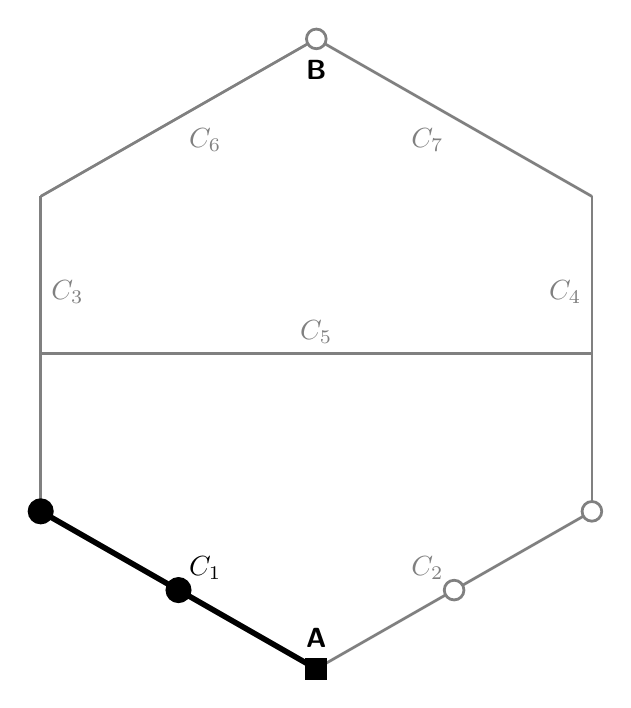
\begin{tikzpicture} [scale=0.5]

\tikzstyle{every path}=[line width=1pt]
\tikzstyle{c1}=[rectangle,minimum size=8]

%\draw[help lines,orange] (-7,-8) grid (7,8);


\draw[gray]  (7,4) -- (7,-4);
\node [above left, gray] at (7,1) {$C_4$};

\draw[gray]  (7,-4) -- (0,-8) ;
\node [above left, gray] at (3.5,-6) {$C_2$};
\draw[gray,fill=white] (7,-4) circle [radius=0.25];
\draw[gray,fill=white] (3.5,-6) circle [radius=0.25];

\draw[gray]  (-7,-4) -- (-7,4);
\node [above right, gray] at (-7,1) {$C_3$};

\draw[gray]  (-7,4) -- (0,8) ;
\node [below right, gray] at (-3.5,6) {$C_6$};

\draw[gray]  (0,8) -- (7,4);
\draw[gray,fill=white] (0,8) circle [radius=0.25];
\node [label=below:$\textsf{\textbf{B}}$, gray] at (0,8) {};
\node [below left, gray] at (3.5,6) {$C_7$};


\draw[gray]  (-7,0) -- (7,0);
\node [above, gray] at (0,0) {$C_5$};

\draw [line width=2pt,black]  (0,-8) -- (-7,-4)
	coordinate[c1,circle, at end,fill=black] (0)
	coordinate[c1,circle,midway,fill=black] (1)
	coordinate[c1,rectangle,at start,fill=black] (2);
\node [above right, black] at (-3.5,-6) {$C_1$};
\node [label=above:$\textsf{\textbf{A}}$, black] at (0,-8) {};

\end{tikzpicture}
\end{center}
\caption{(Color online)
``Bug-type'' \cite{Specker-priv} Greechie orthogonality diagram
with an overlaid two-valued assignment reflecting ``$P(\textsf{\textbf{A}})=1$ implies $P(\textsf{\textbf{B}})=0$.''
This configuration is part of the original
proof of the Kochen-Specker theorem \cite[$\Gamma_1$]{kochen1}.
For concrete coordinatizations, see, for instance, the original paper by Kochen and Specker, as well as Ref.~\cite{svozil-tkadlec,2012-incomput-proofsCJ}.
It is assumed that the system is prepared in state $C_1$, depicted by a block colored in thick filled black;
all the other six remaining contexts $C_2$--$C_7$ are   ``phantom contexts'' colored in gray.
}
\label{2012-psiqm-v2-f2}
\end{figure}

\begin{conjecture}[Context translation principle]
Any mismatch between the preparation and the measurement results in the ``translation''
of the original information encoded by a quantum system into the answer requested.
Thereby stochastic noise is introduced by the many degrees of freedom of a suitable ``quasi-classical'' measurement apparatus.
\end{conjecture}


\begin{definition}[Quantum entanglement]
Any information can be encoded ``across'' compound quanta \cite{zeil-99,zeil-bruk-02,zeil-bruk-99}; thereby inducing entanglement.
\end{definition}
\begin{note}
There appears to be a connection between entangled (i.e., non-factorizable) states with primality:
whenever the dimension of the Hilbert space is prime, there is no way to consider or transform
the system into an entangled state of compound quanta,
because primality implies that the corresponding Hilbert space cannot be decomposed into products of Hilbert spaces.
On the other hand, the uniqueness of the prime factor decomposition implies that any non-prime-dimensional Hilbert space can be perceived
as a unique product of its factors \cite{Schwinger.60,Ellinas-99,Revzen-06,PhysRevA.78.012101,Simkhovich-10},
which thereby refer to ``compound quanta.''
Thereby, the unique prime decomposition
``takes care'' of the possible decomposition into ``compound quanta existing'' in prime-dimensional Hilbert spaces.
\end{note}


\begin{definition}[Quantum state evolution]
A {\em quantum state evolution}
can be represented by a unitary transformation $\textsf{\textbf{U}}$;
that is, by permutations of vectors preserving the inner product (and thus distance, which makes it an isometry).
\end{definition}

\begin{definition}[Stationary state as fixed point]
A {\em stationary state} $ | \psi \rangle$ is a fixed point of the evolution;
that is, $\textsf{\textbf{U}} | \psi \rangle \propto  | \psi \rangle$ .
\end{definition}
\begin{motivation}
For a state to be temporally stationary it has to remain invariant with respect to temporal evolution.
\end{motivation}

\begin{conjecture}
{\em For all practical purposes} (FAPP) \cite{bell-a}  irreversible measurements exist.
FAPP an irreversible measurement need not reflect a property of the ``object;''
it may, for instance, ``come about'' by incomplete knowledge of both the ``object''
and the ``measurement apparatus''  because of too many, uncontrollable degrees of freedom.
\end{conjecture}

\begin{note}
If what is considered as measurement is purely conventional,
then how can one overcome the issue of the quantum co-existence of classically mutually inconsistent information?
Pointedly stated, how come we experience our world in a unique, consistent,
coherent manner when we and everything we observe should be in  coherent superposition?
Schr\"odinger was particularly concerned about
the continuous ``spreading'' of coherent superpositions due to the quantum state evolution.
He first introduced the ``cat paradox'' \cite{schrodinger}, and later mentioned
that {\em ``we should find our surroundings rapidly
turning into a quagmire, or sort of a featureless jelly or plasma, all contours
becoming blurred, we ourselves probably becoming jelly fish
\cite{schroedinger-interpretation}.''}
One radical departure from this conundrum is Everett's relative-state formulation.

Other attempts to cope with ``jellification'' claim the FAPP ``destruction''
of a superposition of macroscopic distinct states
is by the
``environment effectively monitoring'' such a state \cite{RevModPhys.75.715}.
Thereby, no explicit observer needs to be present, because as
Mandel concludes \cite{mandel-operational-cat},
based on an interferometer experiment \cite{zou-wang-mandel:91a,zou-wang-mandel:91b},
``the mere feasibility of the observations, in principle, is sufficient to achieve the same effect, because
the state reflects not only what is known, but also what is knowable in principle.''
This amounts to claiming that FAPP macroscopic superpositions cannot exist.

Alas these attempts  can only be perceived as FAPP applicable;
in a very similar way as in classical statistical mechanics the entropy is increasing FAPP.
There is, for instance, some analogy to Loschmidt's reversibility paradox \cite[p.~139]{Loschmidt}
--
that, for large isolated systems with reversible laws of motion, FAPP  one never
observes a decrease in entropy
--
as well as Zermelo's recurrence objection  \cite[pp.~18ff]{Ebbinghaus-Zermelo}.
\end{note}


\begin{theorem}[No measurement]
In a uniform, surjective (onto),  reversible (one-to-one)  evolution amounting to state permutation,
no irreversible (many-to-one)``measurement'' exists.
\end{theorem}
\begin{proof}
If the (quantum) state evolution is a bijection, it amounts to a permutation.
The symmetric group (of permutations) leaves no room for many-to-one transformations.
In particular, according to Caylay's theorem \cite{jacobson-LoAAI},
the unitary group (as all other groups) acting on states
is isomorphic to some subgroup of the symmetric group acting on on states.
\end{proof}
\begin{note}
As Everett \cite{everett}
pointed out, a uniformly reversible theory never allows irreversible processes such as ``measurement,''
because if one includes the object, the cut and the measurement apparatus (including the environment)
in the reversible description, then this entire system must be reversible.
The question then remains what (if anything) prevents such systems
from quantum jellification  \cite{schroedinger-interpretation}.
This issue can be resolved by the single state conjecture.
\end{note}




\begin{theorem}[Metaphysical fallacy of omni-existence]
The registration of detector clicks associated with outcomes of measurements
does not necessarily reflect a pre-existing observable corresponding to this measurement.
\end{theorem}
\begin{proof}
An exact formalization of value (in)definiteness
of counterfactuals
has been presented in Ref. \cite{2012-incomput-proofsCJ}.
Counterfactuals imply that their ontological
existence can neither be asserted to be necessary nor sufficient by pure empirical evidence alone.
\end{proof}
\begin{note}
By an anecdotal example you may attempt to ask a Viennese where in her city {\it Saint Peter's Basilica} is.
When
--
what is very common among Viennese --
in order not to feel ashamed that she does not know where exactly in Vienna {\it Saint Peter's Basilica} is
(it is nowhere)
--
she presents some (arbitrary) directions,
you will most likely end up at some other church (probably {\it St. Peter's Church}).
Alas this is will not be
{\it Saint Peter's Basilica}
-- one has to travel to Rome for that.
Nevertheless, by analogy, a quantum physicist would claim FAPP existence {\it Saint Peter's Basilica} in Vienna.
\end{note}



\begin{theorem}[No mixed state]
No mixed  state can evolve from a pure state by uniform unitary evolution.
\end{theorem}
\begin{proof}
The proof is based on the same group theoretic argument as the ``no measurement theorem;''
that is, on permutations.
\end{proof}

\begin{theorem}
FAPP a mixed quantum state can evolve from a pure quantum state by incomplete inclusion of the environment.
\end{theorem}
\begin{proof}
The same arguments as for the FAPP existence of irreversible measurements apply.
\end{proof}


\begin{theorem}[Metaphysical fallacy of provable randomness or (in-)determinism]
Empirical randomness can neither be proven nor disproven.
\end{theorem}
\begin{proof}
By reduction (residing in substitution and diagonalization \cite{smullyan-92})
to G\"odel-Tarski-Turing incompleteness, including the recursive unsolvability
of the general rule inference problem,
the general forecast and induction problem
is provable unsolvable for deterministic
(i.e., computable) systems inside that very system \cite{svozil-07-physical_unknowables}.
Thus, it is impossible to either prove or disprove that some system emanating signals such as finite strings of symbols
is either deterministic or indeterministic.
All such claims remain conjectural,
if not religious (cf. Born's confession
\cite{born-26-1,born-26-2}), or ideological.
\end{proof}

\begin{note}
Insofar as context translation is postulated,
randomness is not created {\it ex nihilo} (out of nothing),
and therefore is not irreducible (and in this sense is not ``ontic'').
In this scenario, quantum randomness is the outcome of a rather complex but unitary context translation mechanism,
which, at least in principle, is reducible and resolvable into the many degrees of freedom of the measurement apparatus.
And therefore, epistemic quantum randomness exists FAPP.
\end{note}




\begin{acknowledgments}
 This research has been partly supported by FP7-PEOPLE-2010-IRSES-269151-RANPHYS.
This contribution was done in part during a visiting honorary appointment at the University of Auckland, New Zealand.
Discussions during a {\em LARSIM/QuPa workshop on physics and computation} at the {\it Institut Henri Poincar\'e}, Paris on June 28-29, 2012,
where a previous version of this paper has been presented, are gratefully acknowledged.
I gratefully acknowledge stimulating discussions with Professor Constantine Tsinakis with respect to group theory, and other algebraic issues.
\end{acknowledgments}

 \bibliography{svozil}

\end{document}
